\subsection{Функция Грина уравнения Лапласа первой краевой задачи в круге, на полуплоскости в полупространстве. Метод отражений.}

Функцией Грина (внутренней) задачи Дирихле для (ограниченной) области $G$ называется функция $\mathcal{G}(x, y)$, $x \in \bar{G}$, $y \in G$, обладающая следующими свойствами:
\begin{enumerate}
	\item при каждом $y \in G$ представляется в виде
	\begin{equation}
		\mathcal{G}(x, y) = \frac{1}{4 \pi \abs{x - y}} + g(x, y),
	\end{equation}
	где функция $g(x, y)$ гармоническая в $G$ и непрерыная на $\bar{G}$ по $x$;
	
	\item при каждом $y \in G$ удовлетворяет граничному условию 
	\begin{equation}
		\mathcal{G}(x, y)|_{x \in S} = 0.
	\end{equation}
\end{enumerate}

Для построения функции Грина для области с достаточно широкой симметрией весьма эффективным оказывается \textit{метод отражений}. Продемострируем его на примере шара. 

	Шар $U_{R}$. Пусть $y \in U_{R}$, $y \not = 0$ и 
	\begin{equation} \label{inverse_transform}
		y^{\ast} = y \frac{R^2}{\abs{y}^2}, \quad \abs{y} \abs{y^{\ast}} = R^2,
	\end{equation}
	--- симметричная точка относительно сферы $S_R$ при преобразование инверсии.
	
	Ищем функцию Грина в виде
	\begin{equation} \label{green}
		\mathcal{G}(x, y) = \frac{1}{4 \pi \abs{x - y}} - \frac{\alpha}{4 \pi \abs{x - y^{\ast}}},
	\end{equation}
	где $- \alpha / 4 \pi$ --- неизвестный заряд в симметричной точке $y^{\ast}$. Функция
	\begin{equation*}
		g(x, y) = - \frac{\alpha}{4 \pi \abs{x - y^{\ast}}}
	\end{equation*}
	гармоническая в $U_{R}$. Подберем $\alpha$ так, чтобы $\mathcal{G}(x, y)$ обратилась в нуль на $S_{R}$ (из условий определения функции Грина для данной задачи вытекает, что функция грина образается в нуль на $S$). Для этого заметим, 

	\begin{figure}[H]
		\centering
		\begin{subfigure}{0.4\textwidth}
			\centering
			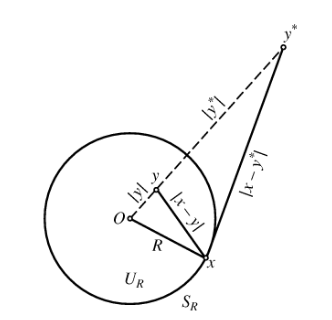
\includegraphics[width=0.7\linewidth]{img/mirror4}
			\caption{}
			\label{img_a}
		\end{subfigure}
		\vspace{5mm}
		\begin{subfigure}{0.4\textwidth}
			\centering
			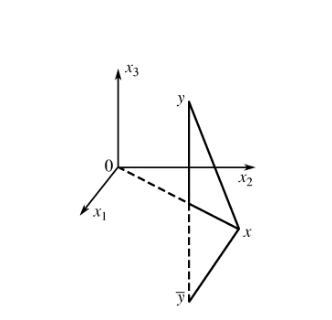
\includegraphics[width=0.7\linewidth]{img/mirror5}
			\caption{}
			\label{img_b}
		\end{subfigure}
		\caption{}
	\end{figure}
	что при $\abs{x} = R$ треугольники $Oxy^{\ast}$ и $Oxy$ подобны: один угол у них общий, а прилегающие стороны в силу \eqref{inverse_transform} пропорциональны (рис. \ref{img_a}). Поэтому при $\abs{x} = R$ справедливо соотношение 
	\begin{equation*}
		\abs{R}{\abs{y}} = \frac{\abs{x - y^{\ast}}}{\abs{x - y}},
	\end{equation*} 
	и, следовательно, в силу \eqref{green} необходимо положить $\alpha = R/\abs{y}$. Итак,
	\begin{equation} \label{ballGreen}
		\mathcal{G}(x, y) = \frac{1}{4 \pi \abs{x - y}} - \frac{R}{4 \pi \abs{y} \abs{x - y^{\ast}}} = \frac{1}{4 \pi \abs{x - y}} - \frac{R \abs{y}}{4 \pi \abs{x \abs{y}^2 - y R^2}}
	\end{equation}
	есть \textit{функция Грина для шара}. Формула \eqref{ballGreen} справедлива и при $y = 0$:
	\begin{equation*}
		\mathcal{G}(x, 0) = \frac{1}{4 \pi \abs{x}} - \frac{1}{4 \pi R}.
	\end{equation*}

	Полупространство $x_3 > 0$ \footnote{Эта область неограничена. Функция Грина в этом случае должна удовлетворять дополнительному условию $\mathcal{G}(x, y) \to 0$ при $\abs{x} \to \infty$, $y \in G$}. Пусть точка $y = (y_1, y_2, y_3)$ лежит в этом полупространстве, $y_3 > 0$. Точка $\tilde{y} = (y_1, y_2, -y_3)$ --- симметричная с $y$ точка относительно $x_3 = 0$ (рис. \ref{img_b}).
	
	Нетрудно проверить, что \textit{функция Грина для полупространства $x_3 > 0$ определяется формулой }
	\begin{equation}
		\boxed{\mathcal{G}(x, y) = \frac{1}{4 \pi \abs{x - y}} - \frac{1}{4 \pi \abs{x - \tilde{y}}}.}
	\end{equation}
	
	Функция Грина для задачи Дирихле на плоскости  представляется в виде
	\begin{equation}
		\mathcal(z, \zeta) = \frac{1}{2 \pi} \ln{\frac{1}{\abs{z - \zeta}}} + g(z, \zeta),
	\end{equation}
	где $g(z, \zeta)$ гармоническая в $G$ и непрерывна на $\bar{G}$ по $z$ и удовлетворяет граничному условию 
	\begin{equation}
		\mathcal{G}(z, \zeta)|_{z \in S} = 0.
	\end{equation}
	
	Пусть теперь $G$ --- односвязная область, ограниченная кусочно гладкой кривой $S$, и $w = w(z)$ --- функция, конформно отображающая область $G$ на единичный круг
	\begin{equation}
		w(z, \zeta) = \frac{w(z) - w(\zeta)}{}
	\end{equation}